%----------------------------------------------------------------------------------------
%	PACKAGES & THEMES
%----------------------------------------------------------------------------------------

\documentclass[8pt]{beamer}

\usepackage{etex}
\mode<presentation> {
\usetheme{Vilanova}
}

\usepackage[english]{babel}
\usepackage[utf8]{inputenc}
\usepackage{array}
\usepackage{graphicx}
\usepackage{booktabs}
\usepackage{amsmath,amssymb,amsthm}
\usepackage{xcolor}
\usepackage{tikz}
\usetikzlibrary{arrows}
\usepackage{pifont}
\usepackage{listings,color}

\definecolor{listcomment}{rgb}{0.0,0.5,0.0}
\definecolor{listkeyword}{rgb}{0.0,0.0,0.5}
\definecolor{listnumbers}{gray}{0.65}
\definecolor{listlightgray}{gray}{0.955}
\definecolor{listwhite}{gray}{1.0}

%----------------------------------------------------------------------------------------
%	TITLE PAGE
%----------------------------------------------------------------------------------------
\title{What's new in one year of OTB?}
\author{}
\date{2017-06-07}

\begin{document}

\begin{frame}
\titlepage
\end{frame}

\begin{frame}
  \frametitle{Orfeo ToolBox 5.6 \textit{Scincinae}}
  \framesubtitle{Released 2016-07-28}

\begin{itemize}
\item MPI pipeline execution
\item Samples extractor and selection for supervised classification
\item Support for Sentinel-1 products (geometric calibration)
\item Improve Monteverdi OTB-applications display \& search bar
\end{itemize}

\end{frame}

\begin{frame}[fragile]
\frametitle{Parallel OTB pipeline with MPI}
  \begin{center}
  \vspace{-0.5cm}
  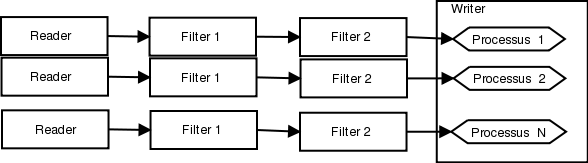
\includegraphics[width=0.6\textwidth]{images/mpi.png}
  \begin{scriptsize}
\begin{verbatim}
    $ mpirun -np $nb_procs --hostfile $PBS_NODEFILE  \
    otbcli_BundleToPerfectSensor \
    -inp $ROOT/IMG_PHR1A_P_001/IMG_PHR1A_P_201605260427149_ORT_1792732101-001_R1C1.JP2 \
    -inxs $ROOT/IMG_PHR1A_MS_002/IMG_PHR1A_MS_201605260427149_ORT_1792732101-002_R1C1.JP2 \
    -out $ROOT/pxs.tif uint16 -ram 1024

    ------------ JOB INFO 1043196.tu-adm01 -------------

    JOBID           : 1043196.tu-adm01
    USER            : michelj
    GROUP           : ctsiap
    JOB NAME        : OTB_mpi
    SESSION         : 631249
    RES REQSTED     : mem=1575000mb,ncpus=560,place=free,walltime=04:00:00
    RES USED        : cpupercent=1553,cput=00:56:12,mem=4784872kb,ncpus=560,vmem=18558416kb,
    walltime=00:04:35
    BILLING         : 42:46:40 (ncpus x walltime)
    QUEUE           : t72h
    ACCOUNT         : null
    JOB EXIT CODE   : 0

    ------------ END JOB INFO 1043196.tu-adm01 ---------
\end{verbatim}
\end{scriptsize}
\end{center}
\end{frame}

\begin{frame}
\frametitle{Orfeo ToolBox 5.8 Sphenomorphinae}
\framesubtitle{Released 2016-11-08}
\begin{block}{OTB}
\begin{itemize}
\item Access to Shark random forests (better performances, parallel learning)
\item Better performances in BandMathX
\item Spot7 support (radiometric and geometric calibration)
\item Applications in-memory connection
\item And lots of other small improvements ...
\end{itemize}
\end{block}

\begin{block}{Monteverdi}
\begin{itemize}
\item Now part of OTB source code
\item Zoom with mouse wheel without CTRL
\end{itemize}
\end{block}
\end{frame}


\begin{frame}
\frametitle{Orfeo ToolBox 5.10 \textit{Valentine}}
\framesubtitle{Released 2017-02-14}
  \begin{block}{OTB}
    \begin{itemize}
      \item Composite applications framework
      \item TrainImagesClassifier and BundleToPerfectSensor refactoring (composite)
      \item Print corresponding command-line in apps QT GUI
      \item Enhancement of field selector QT component
      \item FFT/DWT application
      \item Texture app now allows for subsampled results (faster)
    \end{itemize}
  \end{block}

  \begin{block}{Monteverdi}
    \begin{itemize}
      \item Single band color mapping
      \end{itemize}
  \end{block}

\end{frame}

\begin{frame}
\frametitle{Monteverdi on the fly color mapping}
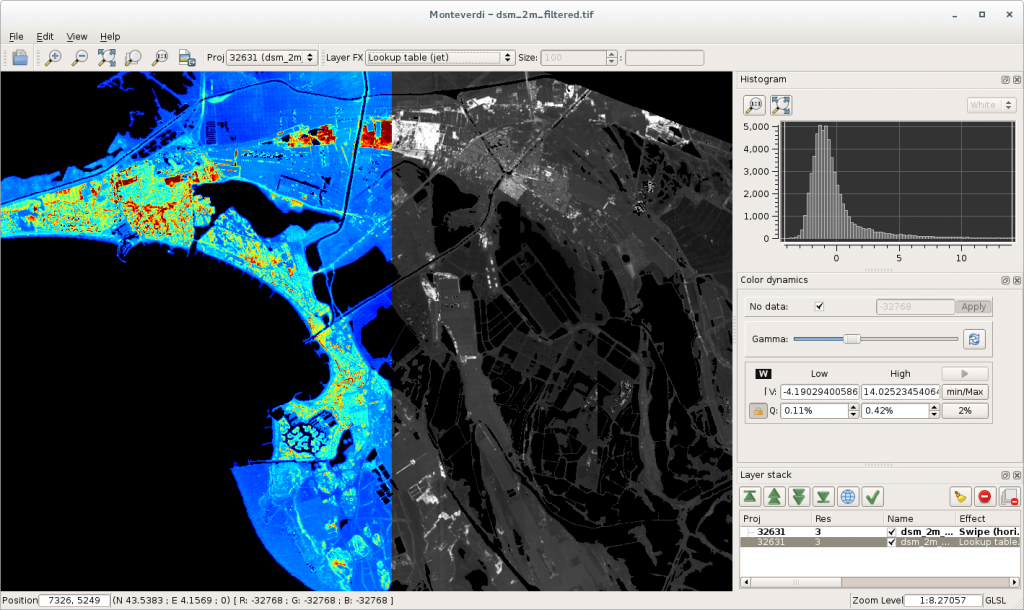
\includegraphics[width=1\textwidth]{images/monteverdi-colormapping.png}
\end{frame}

\begin{frame}
\frametitle{Orfeo ToolBox 6.0}
\framesubtitle{Released 2017-05-15}
  \begin{block}{OTB}
    \begin{itemize}
      \item Licence change to  Apache v2.0
      \item OpenCV 3.0 support
      \item Sentinel1 IW SLC deburst application
      \item Band selection through extended filenames
      \item Unsupervised classification in framework
      \item Morphological profiles app
      \item Vector files classification app
      \item Deprecated code cleanup (major release)
    \end{itemize}
    \end{block}
\end{frame}

\begin{frame}
\frametitle{PSC recuitement}
\end{frame}

\end{document}
